\clearpage
\phantomsection
% \addcontentsline{toc}{chapter}{Chapter 2 -- chapter one title here}
\cftaddtitleline{toc}{chapter}{Chapter 2 -- chapter one title here}{10}

\resetlinenumber

\begin{center}
\textbf{\Large{}Chapter 2 -- chapter one title here}
\label{chap:chapter2}
\par\end{center}{\Large \par}

\bigskip{}


\begin{center}
Your name\textsuperscript{*} and Your advisor
\par\end{center}

\bigskip{}

\lyxaddress{Department of Botany, University of Wisconsin-Madison, Madison, WI,
53706 USA}

Emails: xxx@wisc.edu

{*} Correspondence: Your name, Tel: (608) 265-2191

\chapter*{}
\setcounter{chapter}{2}


\textbf{Abstract:}

Plant community functional traits allow us to mechanistically link changes in species composition to changes in ecosystem functions.

\textbf{\emph{Keywords:}} long-term community assembly; functional
diversity.

\clearpage{}

\phantomsection\addcontentsline{toc}{section}{Introduction}
\section*{Introduction}

Global biodiversity is changing at an unprecedented rate in response to ongoing anthropogenic global environmental changes \citep{sala2000biodiversity}.

\phantomsection\addcontentsline{toc}{section}{Methods}
\section*{Methods}
\subsection*{Study sites and vegetation data}
We re-sampled 30 sites in the central sand plains (CSP) of Wisconsin in 2012 first sampled by James Habeck in 1958.

\phantomsection\addcontentsline{toc}{section}{Results}
\section*{Results}
\subsection*{Changes in environmental conditions}
Both stand characteristics and climatic conditions have changed since 1958. Average canopy cover, average annual precipitation, average annual temperature, and average temperature of the coldest month in these communities have all increased (Fig. \ref{fig:shade_climate_changes}, paired t-tests, all $p\ll0.001$).

\phantomsection\addcontentsline{toc}{section}{Discussion}
\section*{Discussion}
Widespread changes in disturbance regimes make it critical to understand the long-term impacts of disturbance on the taxonomic and functional diversity of plant communities.

\phantomsection\addcontentsline{toc}{section}{Conclusions}
\section*{Conclusions}
These pine barrens communities have increased in local functional diversity while converging in functional composition across sites.

\subsection*{Acknowledgments }
We thank James R. Habeck for his original sampling effort.

\clearpage{}
% \nocite{*}
\begin{onehalfspace}
\phantomsection\addcontentsline{toc}{section}{References}
\bibliographystyle{ecology}
\bibliography{chapter2/ch2}
\end{onehalfspace}

\clearpage{}

\setcounter{table}{0}
\setcounter{figure}{0}

\phantomsection\addcontentsline{toc}{section}{Tables}
\section*{Tables:}
\vspace{60pt}
\begin{table}[h]
\caption{\label{tab:functional-traits-list}List of functional traits used
in this study.}


\centering{}%
\begin{tabular}{>{\raggedright}p{0.2\textwidth}>{\raggedright}p{0.3\textwidth}>{\raggedright}p{0.3\textwidth}>{\raggedright}p{0.2\textwidth}}

\toprule
Trait (Abb.) & Description & Related function & Life-cycle phase\tabularnewline
\midrule
{\small{}Pollination mode (Biotic.Polli)} & {\small{}Biotic or Abiotic} & {\small{}Regeneration strategy} & \emph{\small{}Regeneration}\tabularnewline
{\small{}Leaf nitrogen concentration (LNC)} & {\small{}Total amount of nitrogen per unit of leaf dry mass (\%)} & {\small{}Light capture, photosynthetic rate} & \emph{\small{}Vegetative growth}\tabularnewline
\bottomrule
\end{tabular}
\end{table}

\clearpage{}
\phantomsection\addcontentsline{toc}{section}{Figures}
\noindent\textbf{Figures:}

\noindent \textbf{Figure 1.} Changes in canopy cover, annual average temperature, average temperature of coldest month, and annual precipitation of study sites over time.
\clearpage{}


\begin{figure}
\begin{centering}
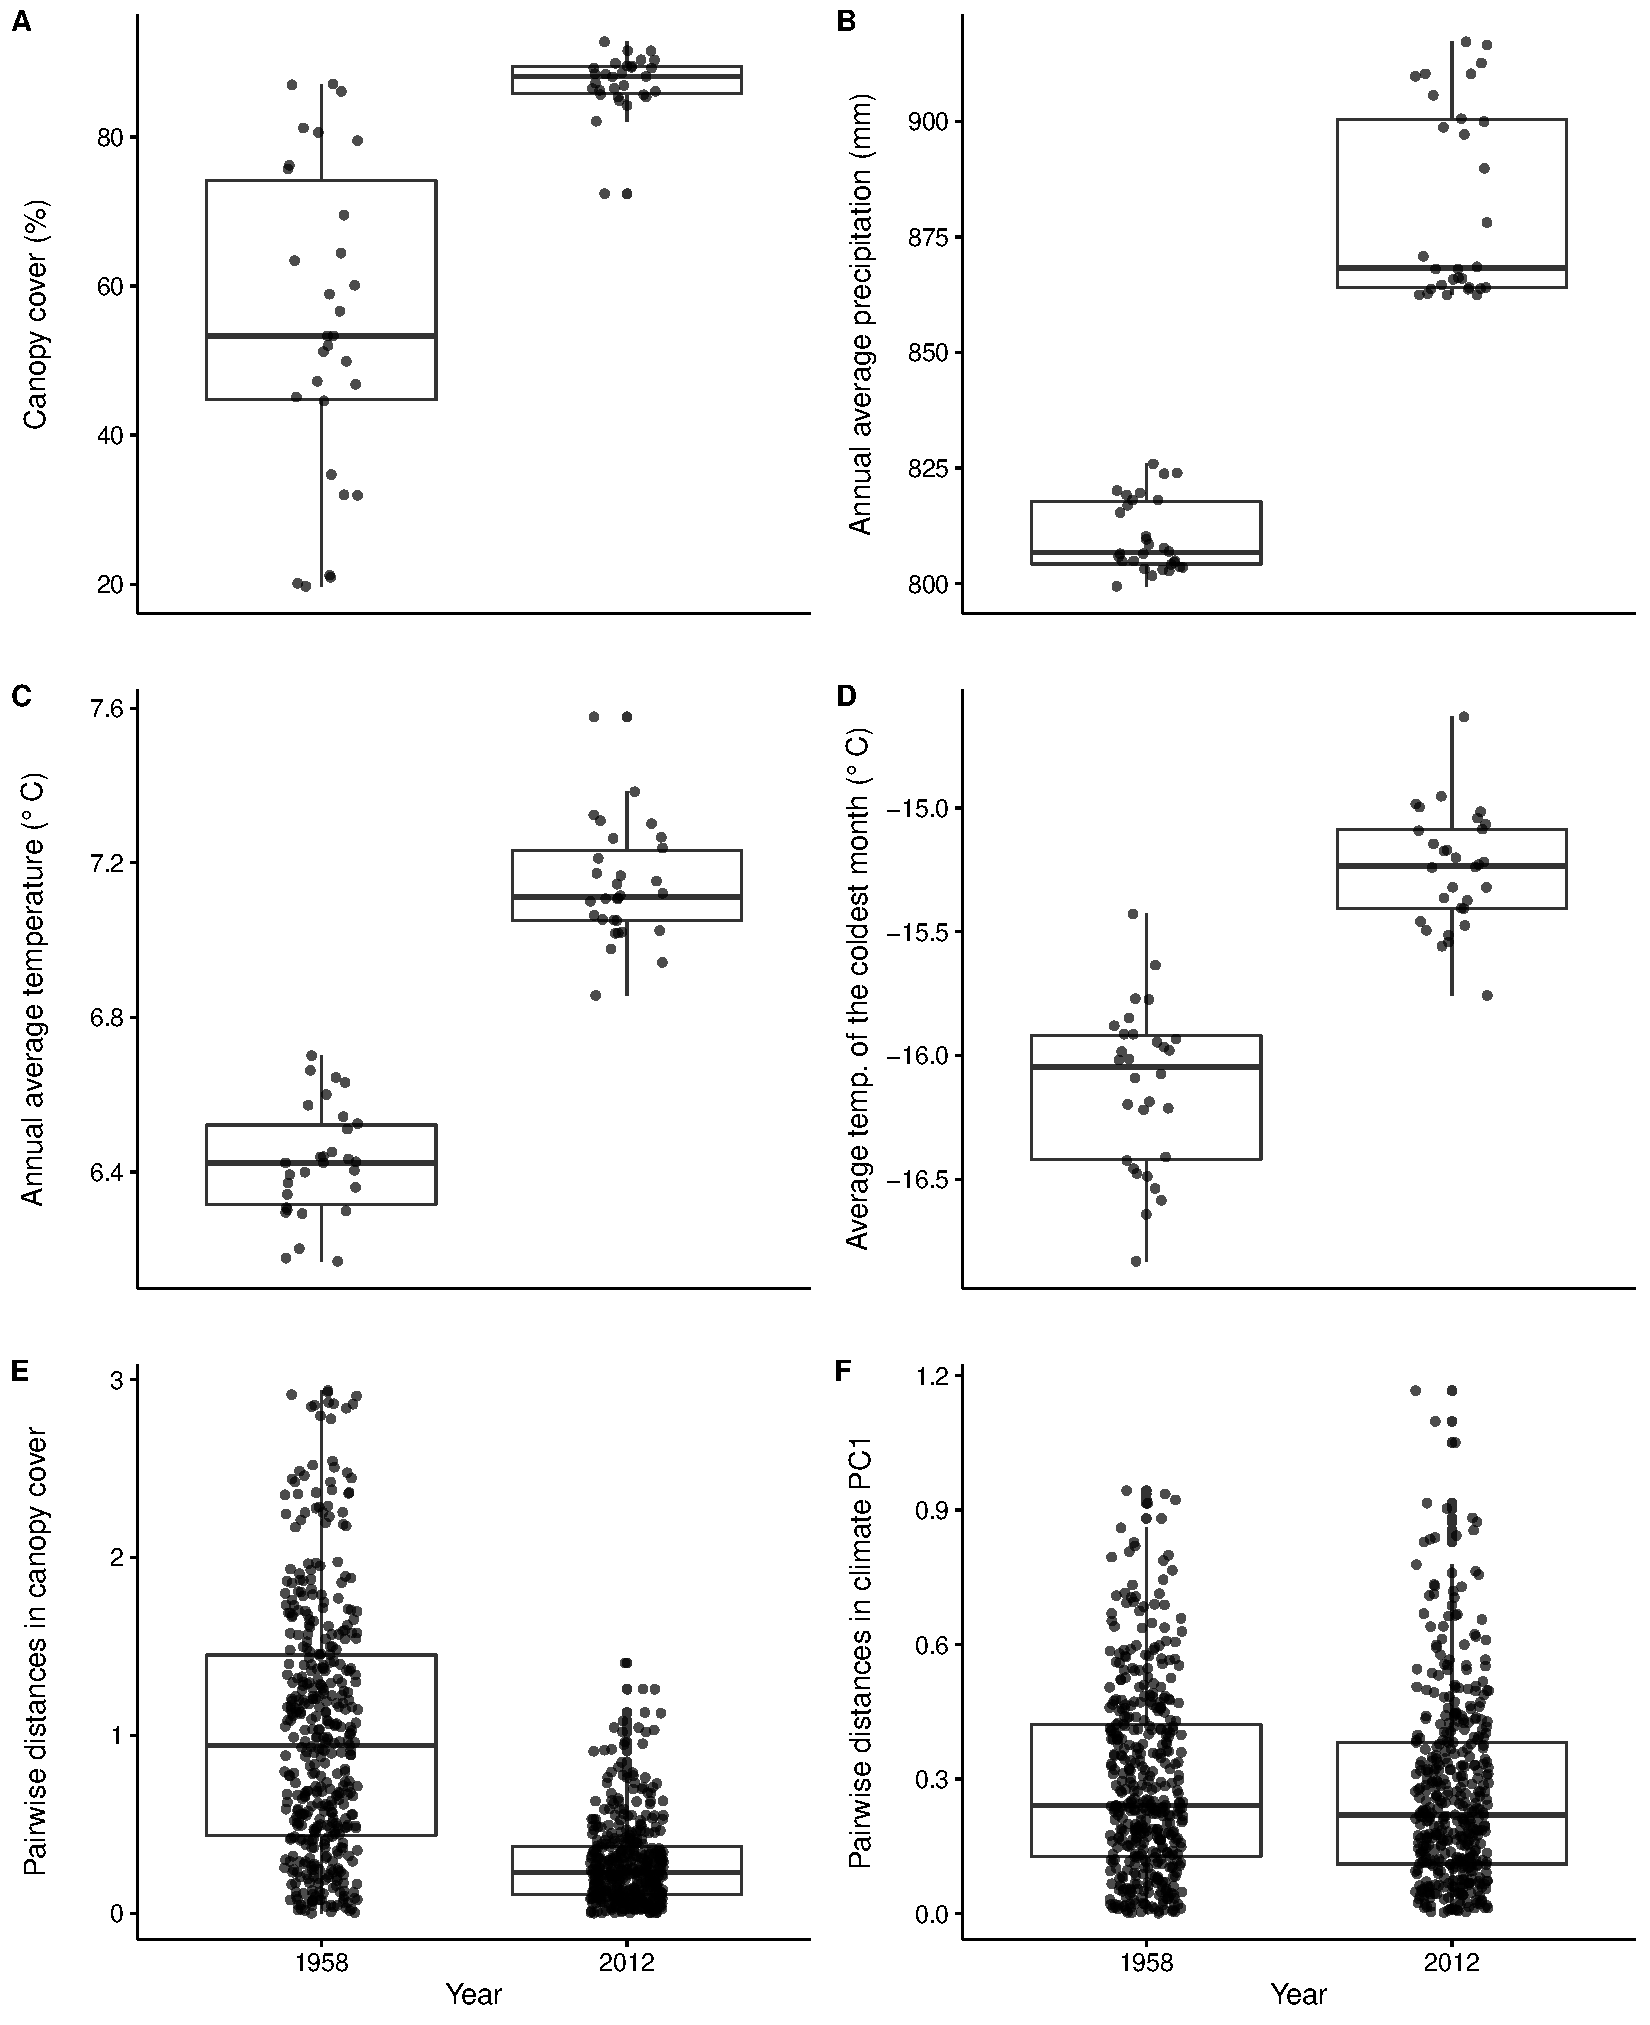
\includegraphics[width=1\textwidth]{chapter2/figures-maintext/shade_climate.pdf}
\par\end{centering}
\caption{\label{fig:shade_climate_changes}
}
\end{figure}

\clearpage{}

\appendix  %%% Appendix %%%%%%%%%%%%%%%%%%%%%%%%%%%%%%%%%%%%%%%%

\renewcommand{\tablename}{\textsc{Table}}
\renewcommand {\thetable}{\textbf{A\arabic{table}}}
\renewcommand{\figurename}{\textsc{Fig.}}
\renewcommand {\thefigure}{\textbf{A\arabic{figure}}}
\setcounter{figure}{0}
\setcounter{table}{0}
\phantomsection\addcontentsline{toc}{section}{Appendix}
\textbf{\LARGE{}Appendix}{\LARGE{}: Supplementary materials.}{\LARGE \par}

\bigskip{}


\textbf{Text A1:} Cumulative proportions and loading of PCA based
on eight climatic variables.\\

\begin{onehalfspace}
\begin{knitrout}
\definecolor{shadecolor}{rgb}{0.969, 0.969, 0.969}\color{fgcolor}\begin{kframe}
\begin{alltt}
\hlkwd{summary}\hlstd{(climate.pca)}
\end{alltt}
\begin{verbatim}
## Importance of components:
##                           PC1     PC2    PC3     PC4    PC5     PC6
## Standard deviation     2.5629 0.88087 0.6499 0.45706 0.1358 0.06558
## Proportion of Variance 0.8211 0.09699 0.0528 0.02611 0.0023 0.00054
## Cumulative Proportion  0.8211 0.91807 0.9709 0.99698 0.9993 0.99982
##                            PC7     PC8
## Standard deviation     0.03344 0.01825
## Proportion of Variance 0.00014 0.00004
## Cumulative Proportion  0.99996 1.00000
\end{verbatim}
\end{knitrout}
\end{onehalfspace}

\begin{figure}
\begin{centering}
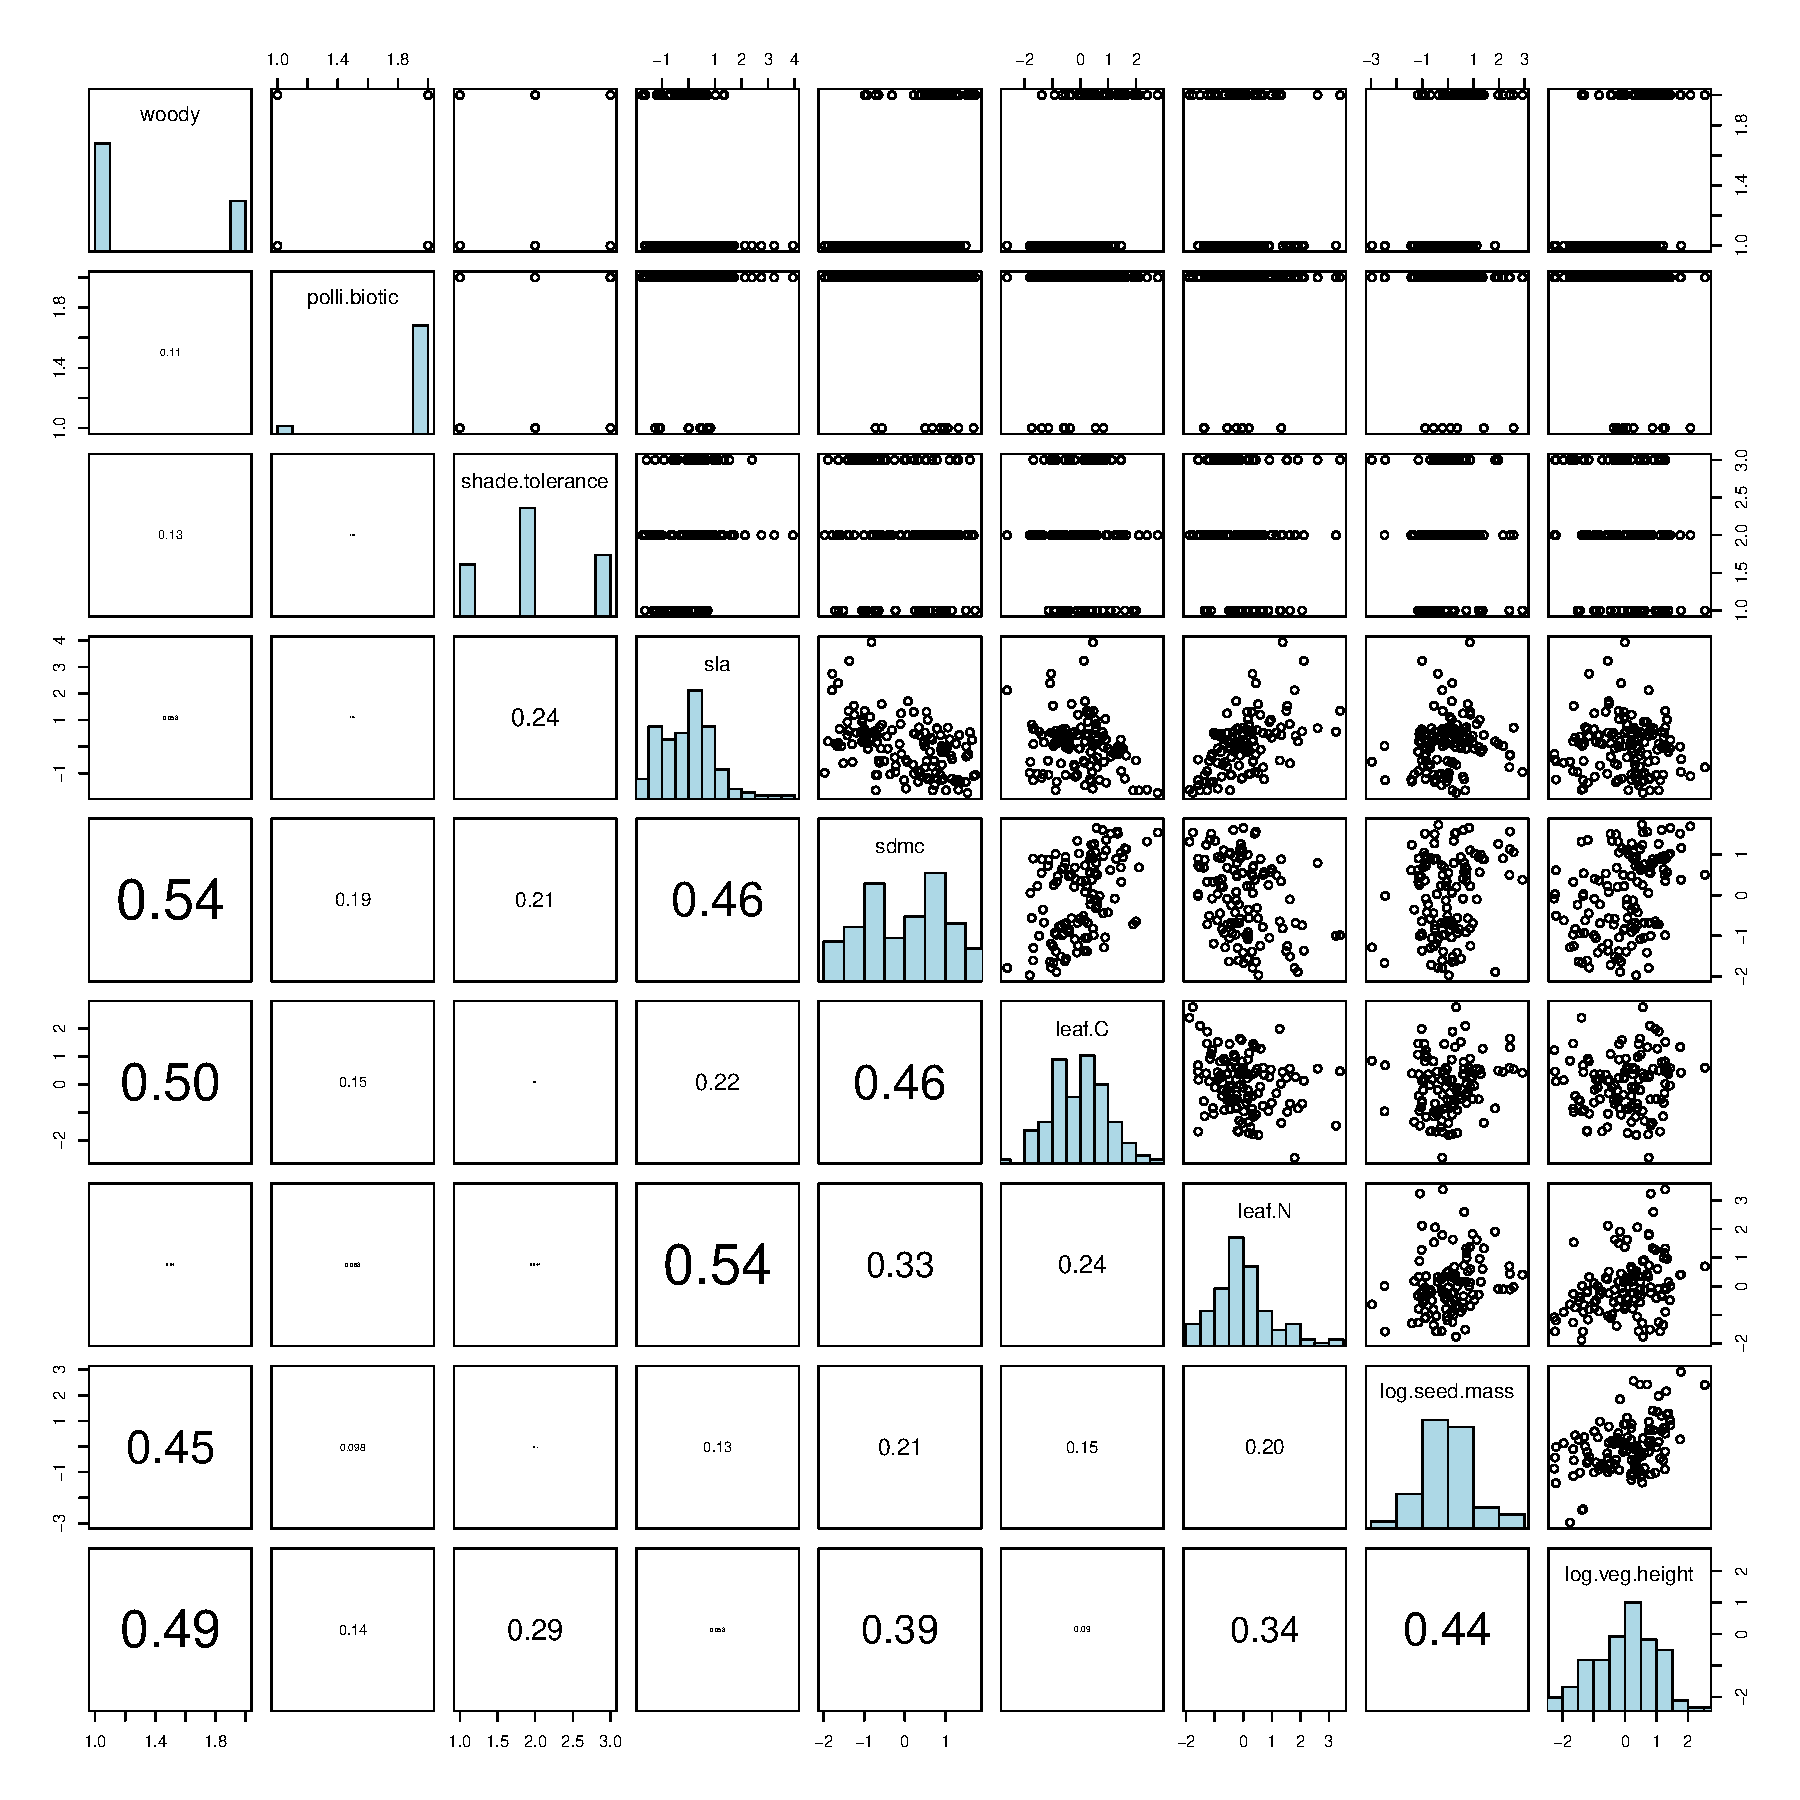
\includegraphics[width=1\textwidth]{chapter2/figures-appendix/trait_cor.pdf}
\par\end{centering}
\caption{Distribution of functional traits used in this study and their pairwise correlations (in absolute value).}
\end{figure}

\renewcommand{\tablename}{Table}
\renewcommand{\thetable}{\arabic{table}}
\renewcommand{\figurename}{Figure}
\renewcommand{\thefigure}{\arabic{figure}}


\clearpage{}
